\documentclass[12pt]{book}
				%这里是导言区

\usepackage{ctex}
\usepackage{amsmath}
\usepackage{graphicx}
\usepackage{url}
\usepackage{listings}
\usepackage{cite}
\usepackage{subfigure}
\usepackage{caption}
% \setmainfont{Caladea}

\lstset{
	frame=shadowbox,
	xleftmargin=2em,
	xrightmargin=2em,
	aboveskip=1em,
	numberstyle=\tiny,
	basicstyle={\ttfamily}
}

\setlength{\oddsidemargin}{0mm}
\setlength{\evensidemargin}{0mm}
\usepackage[left=25mm,right=20mm,top=25mm,bottom=20mm]{geometry}

\linespread{1.25}

\title{基于奇异值变换的航空图像增强}
\author{王佳欣}
\date{2018年5月}

\begin{document}
	\maketitle	 	
	%标题、作者、日期 按照预定的格式展现出来
	\tableofcontents
	
	\chapter{绪论}
		\section{航空图像增强概述}随着航空技术及无人机技术的快速发展,航拍图像成为了现今获取地面观察数据的重要来源。航拍图像在气象观测、国土调查、疫情控制、地理测绘等领域起重大作用。由于环境污染加重以及恶劣天气的存在,社会对航空图像的质量提出了更高的要求。例如,在沙尘、雾霾等天气条件下,图像采集设备难以获得清晰图像以便后续工作的开展。因此开展对航空图像的增强话处理意义重大。%\\ \indent
		
本课题针对模糊不清、对比度低的灰度航空图像,提出了基于奇异值分解和二维离散小波变换的图像增强处理。并通过主观评价和诸如平均值、标准差、直方图的客观评价指标进行评价。.
		\section{航空图像的特点}
			\subsection{航空图像特点}任何物体都有不同的电磁波反射和辐射特征,遥感技术是利用飞机等飞行器或者人造卫星对反射和辐射特征进行采集和分析,探测、分析和识别特定对象的技术。根据采集平台分类,遥感可以分为地面遥感、航空遥感和航天遥感;根据电磁波波长分类,遥感可分为微波遥感、红外遥感和可见光近红外遥感。由于航空遥感具有机动灵活且免受云层干扰等诸多优点,因此本文中所有的实验数据都采用“航空遥感图像”(简称为“航空图像”),更具体地,本研究中所说的航空图像指在飞机上拍摄的航拍图像,航拍图像有以下优点\cite{?}:
				\begin{itemize}
					\item \emph{航空图像信息容量大,空间分辨率大。}
					\item \emph{航拍图像应用灵活。可灵活的设置图像分辨率以及采集频率等信息,另航空图像在空间以及时间上具有较强的灵活性,有利于制定合适的方案。}
					\item \emph{航空图像信息的获取方便。}
				\end{itemize}

			 但是航拍图像也有受环境信息干扰大、勘探范围有一定的局限性的缺陷。
			\subsection{图像增强的意义}图像增强作为图像处理的一个古老而重要的分支,在不断地应用需求变化面前,也在不断更新其研究目标和发展其增强处理方法技术。通常,由于场景本身所包含的动态范围、光照条件、图像捕获设备如数码相机的局限,以及摄影者本身的技术问题等多种因素影响,多数情况下,会使得拍摄的图像达不到人们预期的目标,如场景中的运动目标产生的运动模糊、由于曝光不恰当引起的场景细节损失或是弱小目标辨识不清等,都会对后期的图像前后景分割、目标识别、目标跟踪和最终的图像理解以及预测分析等带来困难。而图像增强本身的目标就是为了突出图中感兴趣的区域、降低或去除不需要的图像信息,以此来加强和获取用户觉得有用的信息,进而得到更加适合于人/机器对图像进行理解和分析处理的表现形式或是富含更多细节信息的图像的相应处理方法\cite{?}。
			\subsection{国内外研究现状}
			
			\subsection{本文主要内容与结构}本文提出基于奇异值与二维离散小波变换的灰度航空图像增强,并通过实验证明本文所提出的方法的有效性。本文的具体结构安排如下:

第一章,绪论。介绍本课题的研究背景和意义,分析了航空图像的特点及其图像增强的意义。

第二章,
	\chapter{常用的图像增强方法}本章首先介绍直方图均衡增强算法和Retinex增强算法的基本原理和发展历程,阐述他们在航空图像增强中的应用。	
		\section{直方图均衡增强算法}直方图描述了一幅图像的绘图统计信息,是一个关于灰度的函数,如令$x$表示灰度值,则离散函数$f(x)$表示当$x$为特定灰度值时,一幅图像上灰度值为$x$的像素的数量。

直方图均衡属于图像增强技术中的空域方法,即直接对像素值施加以相应的操作以获得增强效果。直方均衡是一种利用图像的直方图像来调整图像对比度的一项技术,该技术基于将原场景图像的直方图经重新映射后得到一个接近于均匀分布的概率密度函数的新的直方图的思想,是一种简单有效的对比度拉伸技术\cite{?}。	

直方图均衡的目的是使原始图像原有的灰度分布即直方图,重新在一定的范围内“均匀”分布。而对于原始图像直方图具有的谷值和峰值,直方图均衡处理后仍具有原来的形状,并且变得平滑。以下将阐述直方图均衡的数学表达。

考虑连续的灰度值,用r表示原始出翔的灰度。假设r的取值区间是$[0,L-1]$,灰度值变换公式为
\begin{equation}s=T(r),0 \leq r\leq L-1 \end{equation}
%\begin{eqnarray*}
%x^n+y^n &=& z^n \\
%x+y &=& z
%\end{eqnarray*}
%其中两个&号之间的是公式间对齐的位置,用\\隔开各行公式。上面输出的公式是没有编号的,如果需要自动编号,可以将eqnarray*改为eqnarray 。 

灰度变换公式满足以下条件
			\begin{itemize}
				\item \emph{$T(r)$在区间$0\leq r\leq L-1$上为单调递增函数。}
				\item \emph{当$0\leq r\leq L-1$时,$0\leq T(r) \leq L-1$。}
			\end{itemize}

原始图像的灰度值可视为$[0,L-1]$内的随机变量。用概率密度函数(probability density function,PDF)来描述这些随机变量。有如下公式:
\begin{equation}p_s(s)=p_r(r)|\frac{dr}{ds}|\end{equation}	
其中$p_r(r)$表示随机变量$r$的概率密度函数,$p_s(s)$表示随机变量$s$的概率密度函数。并有如下公式:
\begin{equation}     s=T(r)=(L-1)\int_0^r p_r(v)\,dv    \end{equation}	
\begin{equation}     \frac{ds}{dr}=\frac{dT(r)}{dr}=(L-1)\frac{d}{dr}\left[\int_0^r p_r(v)\,dv 	\right]=(L-1)P_r(r)     \end{equation}
\begin{equation}     p_s(s)=p_r(r) \left| \frac{dr}{ds}\right| =p_r(r) \left| \frac{1}{(L-1)p_r(r)} \right| = \frac{1}{L-1},0 \leq s \leq L-1    \end{equation}
其中,v是积分假变量。公式的右边是随机变量$r$的累计分布函数(cumulative distribution function, CDF)。由公式$(2.5)$得知得到的$p_s(s)$始终是均匀的,与$P_r(r)$无关。简单的来说就是使原始图像的灰度直方图的累计分布函数均匀分布使得原始图像的对比度变高。以下是一个直方图均衡的例子:
			\begin{figure}[!ht]\centering
				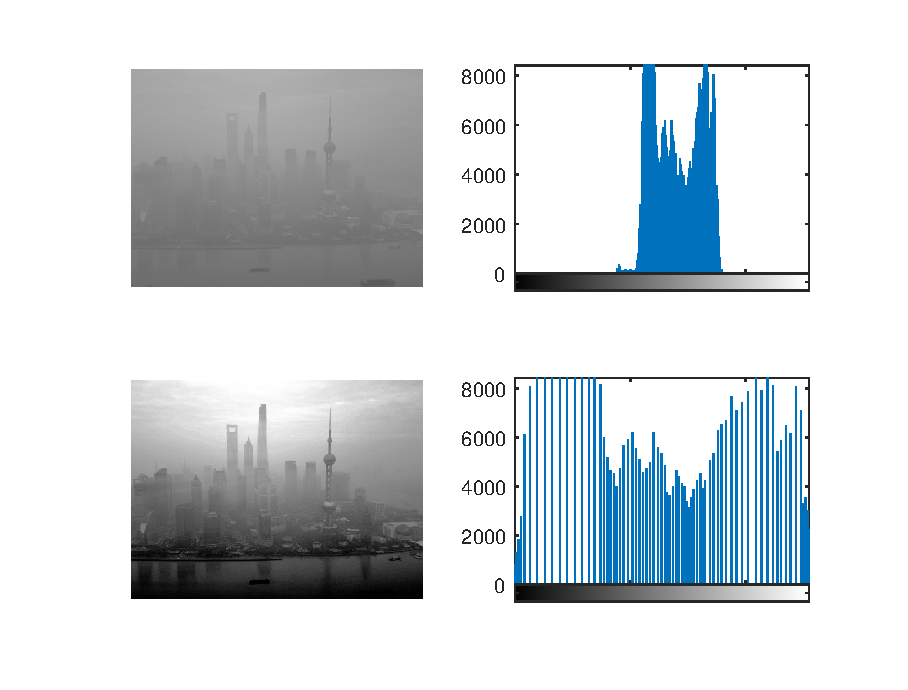
\includegraphics[totalheight=60mm]{./figures/histogramExample.eps}
				\caption{直方图均衡\label{histogram}}
			\end{figure}
从上图可以看出原本对比度很低,模糊不清的原始图像经过直方图均衡后变得更为清晰,视觉效果好。其中,均衡化后图像的灰度直方图形状与原图的灰度直方图相似,只不过被“拉伸"了。直方图均衡有助于图像的增强,但是也有过增强和细节变得更加模糊的缺点。
		\section{Retinex增强算法}	Retinex(Retina-Cortex)理论是在1977年由Edwin Land提出的关于图像增强的理论,器阐述了人通过亮度感知捕捉色度图像在不同亮暗情况下辨认物体的能力。是研究人员模仿人类视觉系统而发展而成的算法,从单尺度Retinex(Single Scale Retinex,ssr)算法改进成多尺度加权平均的Retinex算法(Multi Scale Retinex,msr),再发展成彩色恢复多尺度Retinex算法。一下详细介绍单尺度Retinex算法。

一幅给定图像$s(x,y)$可以分解为两个不同的图像:反射图像$r(x,y)$和亮度图像$L$,原理图如下:
			\begin{figure}[!ht]\centering
				\includegraphics[totalheight=60mm]{./figures/retinexSSR.png}
				\caption{SSR原理图\label{SSR}}
			\end{figure}

如上图所示,入射光照射在反射物体上,通过反射物体的反射形成反射光进入人眼,得到人所见到的图像,用公式表达为:
\begin{equation}     S(x,y)=R(x,y)L(x,y)    \end{equation}	
其中,$L(x,y)$表示入射图像,他决定了图像中像素多能达到的动态范围,$R(x,y)$表示物体的反射性质图像,即图像的内在属性,$S(x,y)$表示人眼所能接收到的反射光图像。该理论的基本思想是在原始图像中,通过某种方法降低或去除入射图像的影响,从而尽可能保留物体本质的反射属性图像。其一般处理过程如下所示:
			\begin{figure}[!ht]\centering
				\includegraphics[totalheight=30mm,width=160mm]{./figures/retinexSSR1.png}
				\caption{SSR原理图(这个图像要改)\label{SSR}}
			\end{figure}

我们把照射图像假设为空间平滑图像,可得单尺度Retinex算法公式为:
\begin{equation}     r(x,y)=logR(x,y)=log \frac{S(x,y)}{L(x,y)}    \end{equation}
\begin{equation}     r(x,y)=logS(x,y)-log \left[ F(x,y)*S(x,y) \right]    \end{equation}	
\begin{equation}     F(x,y)=\lambda e^{\frac{-(x^2+y^2)}{c^2}}    \end{equation}	

其中,$r(x,y)$为输出图像,$*$为卷积符号,$F(x,y)$为中心环绕函数,$c$表示高斯环绕尺度,$\lambda$是一个尺度,中心环绕函数$F(x,y)$的取值要满足
\begin{equation}     \int\int F(x,y)\,dx \,dy=1    \end{equation}

可以从上面的式子中看出SSR算法中的卷积可以看作是对空间中照度图像的计算,它的物理意义可以表示为通过计算图像中像素点和周围区域在加权平均来估计图像中照度的变化,并将其去除,最后只保留图像中物体的反射属性,从而达到增强的目的。中心环绕函数$F(x,y)$采用低通函数,能够在算法中估计出照射图像所对应的原始图像的低频部分,留下对应的高频部分即边缘信息。所以SSR算法可以较好的增强图像中的边缘信息。以下将展示SSR算法的增强效果。
			\begin{figure}[!ht]\centering
				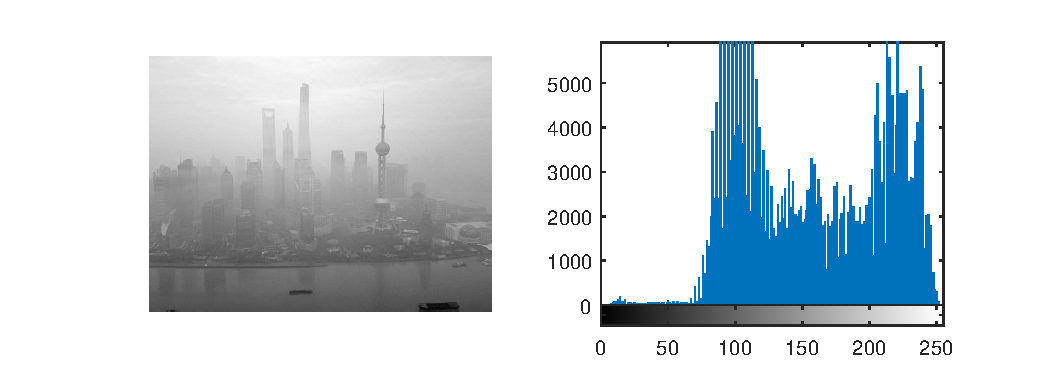
\includegraphics[totalheight=60mm]{./figures/ssr2.eps}
				\caption{SSR增强算法\label{SSR}}
			\end{figure}

从上图中可见,图2.4增强效果好,突出了图像细节,符合人眼感官。从图2.4的灰度直方图中可见,图中形状和图2.1中的灰度直方图相似,对比度加强,即同样被更加适当的“拉伸”了。
	\chapter{DWT-SVD增强算法}这里是概括
		\section{奇异值分解算法}SVD是最小二乘意义下的最优矩阵分解,它将最大信号能量尽可能地分解为尽可能少的系数。奇异值分解(Singular Value Decomposition, SVD)是一种稳定而有效的方法,将系统分解为一组线性无关的分量,每个分量都对系统有一定程度上的贡献。奇异值分解是数值分析中用于对角化矩阵的数值技术。由于SVD具有无穷无尽的优点,如压缩中,在两个独特的子空间数据和噪声子空间的基础上处理图像的能力,所以SVD是一种有吸引力的图像处理代数变换,它通常用于噪声过滤,也被用于水印应用。这些应用程序中的每一个都利用了SVD的关键属性。奇异值分解是鲁棒可靠的正交矩阵分解方法,这是由于其概念和稳定性原因在信号处理领域越来越流行。本文主要介绍奇异值在图像增强的的应用。以下介绍奇异值分解的数学表达。
			\subsection{奇异值分解的数学表达}在线性代数中,SVD是矩阵实数或复数矩阵的分解,类似于使用特征向量的基础的对称或厄密特矩阵的数量化。 SVD是将系统分解为一组线性独立分量的稳定且有效的方法,具有$N \leq M$的尺寸为$M×N$的数字图像$X$可以通过其如下的SVD来表示;
\begin{equation}	\left[ X \right] _{N×M}=\left[ U \right] _{M×M} \left[ S \right] _{M×N} \left[ V \right] ^T_{N×N}	\end{equation}			
\[ U=[u_1,u_2....u_m],	V=[v_1,v_2....v_n] \]
\[
S
=\begin{bmatrix}
s_1  &  0  & \cdots\ &0\\
0  &  s_2  & \cdots\ & 0\\
 \vdots   & \vdots & \ddots  & \vdots  \\
 0 & 0  & \cdots\ & s_n\\
\end{bmatrix}
\]

其中$U$是$M×M$的正交矩阵,$V$是$N×N$的正交矩阵,$S$是$M×N$的矩阵,并且对角元素$s_i$是矩阵$X$的奇异值,下标$T$表示矩阵的转置。正交矩阵$U$的列被称为左奇异向量(Left Singular Vector, LSV),正交矩阵$V$的列被称为右奇异向量(Right Singular Vector, RSV)。$X$的左奇异向量是$XX^T$的特征向量,$X$的右奇异向量是$X^TX$的特征向量。每个奇异值(singular value,SV)指定图像层的亮度,而相应的奇异向量指定图像的几何形状。 U和V是正交矩阵(每列的平方和是独立的,且每个列互不相关),$S$是奇异值递减的对角矩阵。%每个特征图像的奇异值就是它的2-范数。因为SVD使最大奇异值最大化,所以第一特征图像是占最大量的方差 - 协方差结构的模式

		小波变换-数字图像处理p320
		\section{小波变换理论}在数值分析和功能分析中,离散小波变换(Discrete Wavelet Transform, DWT)是对任何小波进行离散采样的小波变换。 。小波变换的基本思想是可变窗口的平移和伸缩的基本思想。Haar基是一种最简单的小波基,具有不连续性的特点。小波变换能自动调节频率窗口和时间窗口并能使频域和时域同时进行局部变换,这一特点是小波变换优于傅里叶变换的地方。小波的特点有:长度有限,均值为零。小波变换能够使用伸缩和平移的特性从多个角度细化目标函数。
			\subsection{离散小波变换}二维离散小波变换是连续信号离散化后的小波变换,可以用来分析诸如图像的二维离散信号,并在图像压缩领域,数字水印领域,图像融合领域皆有所应用。本文着重强调其在图像增强上的应用。DWT示意图图如下所示:
				\begin{figure}[!ht]\centering
					\includegraphics[totalheight=40mm,width=160mm]{./figures/DWT.jpg}
					\caption{DWT二级小波变换分解图\label{DWT}}	
				\end{figure}		

其中,$L$是高低滤波器,$H$是高通滤波器。原始图像经过以及分解后会得到$LL_1$、$HL_1$、$LH_1$、$HH_1$四个子带,子带即一幅图像被分解为一组频带受限的分量,并且子带可以重组在一个构成无误差的原始图像。$LL_1$是水平及垂直方向上的低频子带,$LH_1$是水平方向上低频并且垂直方向上高频的子带,$HL_1$是水平方向上高频并且垂直方向上低频的子带,$HH_1$是水平及垂直方向上都高频的子带。而$LL_2$、$HL_2$、$LH_2$、$HH_2$是子带$LL_1$再次进行一次DWT运算的子带。现在以第一次小波分解为例,进行演示。
				\begin{figure}[ht]
					\begin{minipage}{0.48\linewidth}
						\centerline{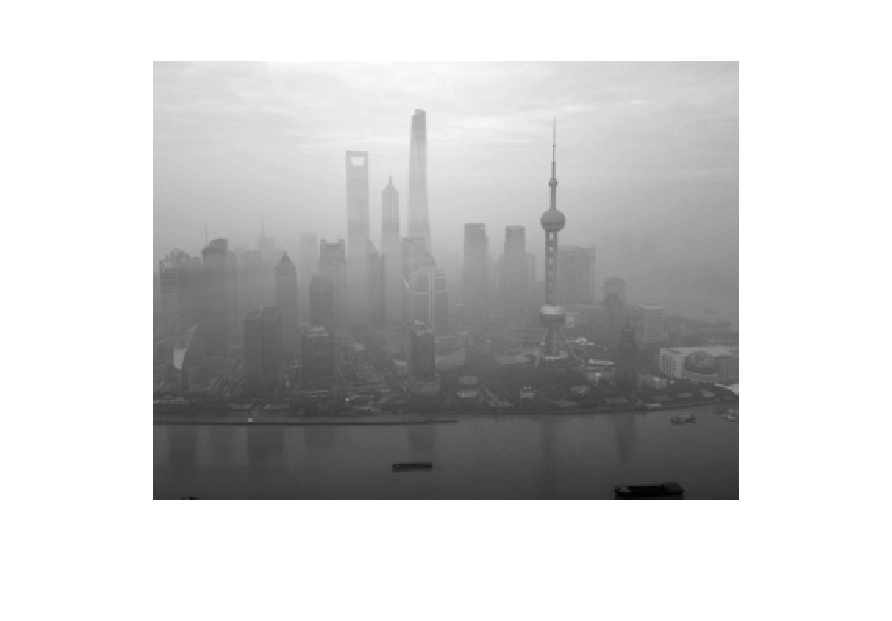
\includegraphics[width=1\textwidth]{./figures/LL.eps}}
						\centerline{LL}
					\end{minipage}
					\qquad
					\begin{minipage}{0.48\linewidth}
						\centerline{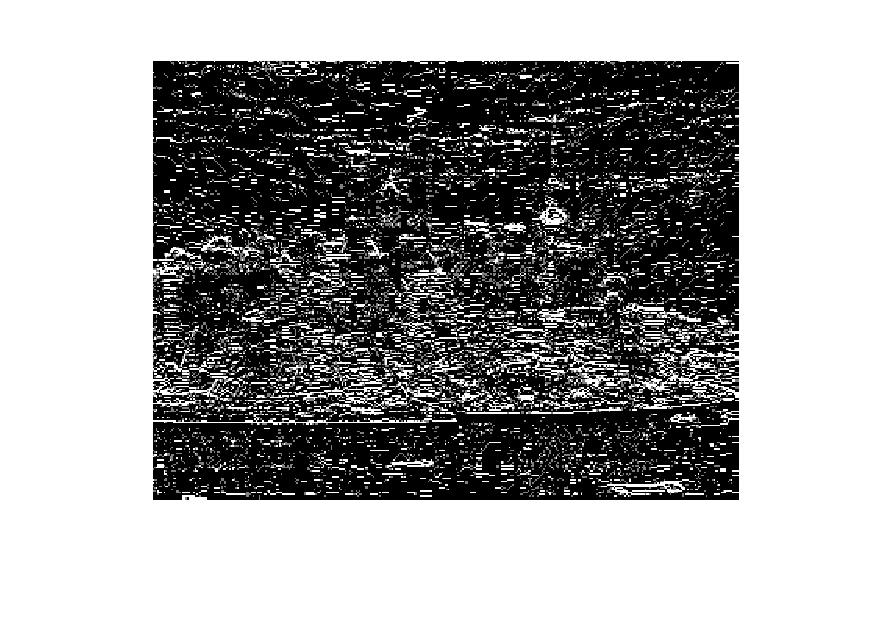
\includegraphics[width=1\textwidth]{./figures/HL.eps}}
						\centerline{HL}
					\end{minipage}

					\begin{minipage}{0.48\linewidth}
						\centerline{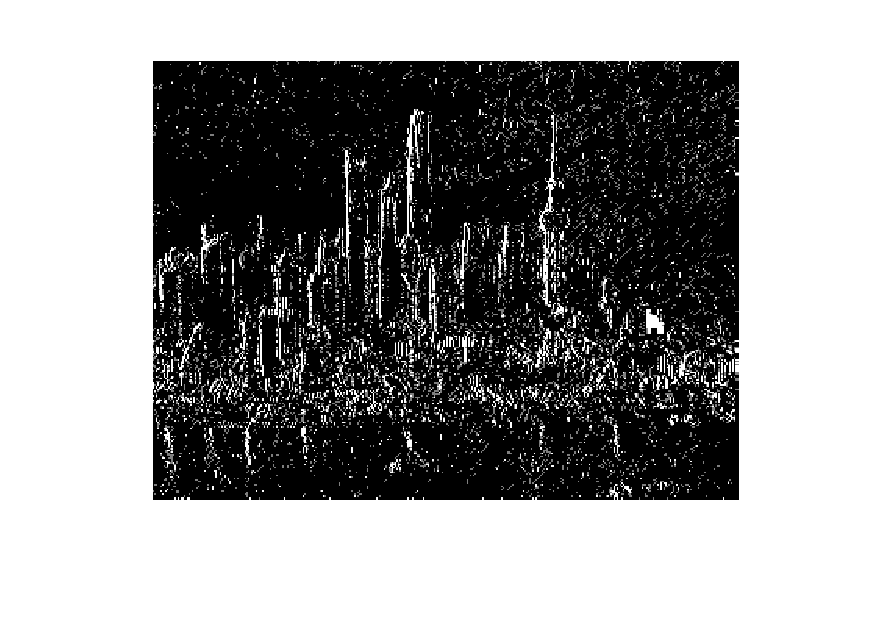
\includegraphics[width=1\textwidth]{./figures/LH.eps}}
						\centerline{LH}
					\end{minipage}
					\qquad
					\begin{minipage}{0.48\linewidth}
						\centerline{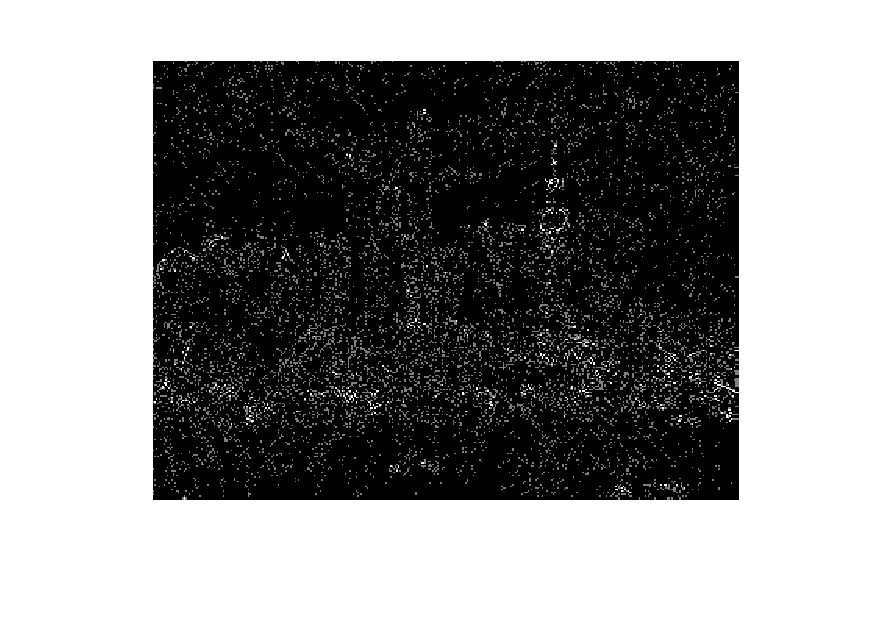
\includegraphics[width=1\textwidth]{./figures/HH.eps}}
						\centerline{HH}
					\end{minipage}
					\caption{DWT示例\label{DWT}}
				\end{figure}

下一步:LL=0矩阵 然后融合
dwt:轮廓保留  
svd:内容增强

		\section{DWT-SVD算法}本文提出的DWT-SVD算法分成为两个部分第一个部分是使用
	\chapter{实验结果及分析}指标

	\chapter{总结}




\end{document}